\documentclass[bachelor,oneside,winfonts]{njuthesis}
\usepackage{epsfig}
\usepackage[linesnumbered,ruled,vlined]{algorithm2e}
\usepackage{amsmath}
\usepackage[noend]{algpseudocode}
\usepackage{tikz}
\SetKwBlock{Begin}{Upon}{end}
\makeatletter
\def\BState{\State\hskip-\ALG@thistlm}
\makeatother
\usepackage{diagbox}


%%%%%%%%%%%%%%%%%%%%%%%%%%%%%%%%%%%%%%%%%%%%%%%%%%%%%%%%%%%%%
% 设置论文的中文封面

% 论文标题,不可换行
\title{面向Redis list的OT函数的设计与验证}
% 如果论文标题过长,可以分两行,第一行用\titlea{}定义,第二行用\titleb{}定义,将上面的\title{}注释掉
%\titlea{分布式移动计算中数据共享技术研究}
%\titleb{}

% 论文作者姓名
\author{纪业}
% 论文作者联系电话
\telphone{18362917059}
% 论文作者电子邮件地址
\email{451686157@qq.com}
% 论文作者学生证号
\studentnum{141220044}
% 论文作者入学年份(年级)
\grade{2014}
% 导师姓名职称
\supervisor{魏恒峰~讲师}
% 导师的联系电话
\supervisortelphone{}
% 论文作者的学科与专业方向
\major{计算机应用}
% 论文作者的研究方向
\researchfield{分布式算法}
% 论文作者所在院系的中文名称
\department{计算机科学与技术系}
% 论文作者所在学校或机构的名称。此属性可选,默认值为``南京大学''。
\institute{南京大学}
% 论文的提交日期,需设置年、月、日。
\submitdate{2018年6月20日}
% 论文的答辩日期,需设置年、月、日。
\defenddate{2018年6月7日}
% 论文的定稿日期,需设置年、月、日。此属性可选,默认值为最后一次编译时的日期,精确到日。
%% \date{2013年5月1日}

%%%%%%%%%%%%%%%%%%%%%%%%%%%%%%%%%%%%%%%%%%%%%%%%%%%%%%%%
% 设置论文的英文封面-

% 论文的英文标题,不可换行
\englishtitle{Design and Verification of OT Function for Redis List}
% 论文作者姓名的拼音
\englishauthor{Ji Ye}
% 导师姓名职称的英文
\englishsupervisor{Reasearch Assistant Wei Henfeng}

% 论文作者学科与专业的英文名
\englishmajor{Computer Application}
% 论文作者所在院系的英文名称
\englishdepartment{Department of Computer Science and Technology}
% 论文作者所在学校或机构的英文名称。此属性可选,默认值为``Nanjing University''。
\englishinstitute{Nanjing University}
% 论文完成日期的英文形式,它将出现在英文封面下方。需设置年、月、日。日期格式使用美国的日期
% 格式,即``Month day, year'',其中``Month''为月份的英文名全称,首字母大写;``day''为
% 该月中日期的阿拉伯数字表示;``year''为年份的四位阿拉伯数字表示。此属性可选,默认值为最后
% 一次编译时的日期。
\englishdate{\today}


\begin{document}
	
	% 制作中文封面
	\maketitle
	% 制作英文封面
	\makeenglishtitle
	
	%%%%%%%%%%%
	% 开始前言部分
	\frontmatter
	
	%摘要
	%%%%%%%%%%%%%%%%%%%%%%%%%%%%%%%%%%%%%%%%%%%%%%%%%%%%%%%%%%%%%%%%%%%%%%%%%%%%%%%
% 论文的中文摘要
\begin{abstract}
	\par 协同编辑系统,可以允许不同地点的用户同时编辑同一份文档。为了获得较快的响应和较高的实用性,系统会在不同的地点或设备进行文档的复制。一个用户可以在某个副本上进行文档的编辑,并将做出的修改异步地传递给其他副本。不必要等待服务器处理完再响应用户操作,本地操作可以立即执行。同时系统必须保证编辑的一致性,即在所有用户完成文档的编辑后,所有的副本内容一致。
	\par 可以设计OT函数,并通过控制算法的调用来保证最终结果的一致性,现在ins,del,set等简单operation的OT函数已经基本实现,本次毕业设计的目标是实现Redis List所支持的14种非阻塞操作的OT函数,并且对实现函数的正确性进行验证。阿里云和RedisLab的团队目前都在对Redis List的操作进行开发,Redis List操作的OT函数实现具有应用前景和商业前途。
	\par 针对上述问题,本文的贡献包括:
	\par 首先介绍了Redis List的相关命令,并将Redis List的相关命令进行基于坐标和操作方式的分类,能够更方便地实现OT函数的设计。
	\par 其次对于所有简化后的命令进行了OT函数的数学公式设计。
	\par 最后介绍了TLA +,并通过TLA+实现了对于所设计OT函数的证明,以及对实验结果的分析。
	% 中文关键词。关键词之间用中文全角分号隔开,末尾无标点符号。
	\keywords{协同编辑;操作转换;Redis 系统;TLA+验证}
\end{abstract}

%%%%%%%%%%%%%%%%%%%%%%%%%%%%%%%%%%%%%%%%%%%%%%%%%%%%%%%%%%%%%%%%%%%%%%%%%%%%%%%
% 论文的英文摘要
\begin{englishabstract}
\par To be filled.
	% 英文关键词。关键词之间用英文半角逗号隔开,末尾无符号。
	\englishkeywords{}
\end{englishabstract}
	
	%%%%%%%%%%%%%%%%%%%%%%%%%%%%%%%%%%%%%%%%%%%%%%%%%%%
	% 生成论文目次
	\tableofcontents
	
	%%%%%%%%%%
	% 开始正文部分
	\mainmatter
	
	
	%前言
	\chapter{前言}
\section{应用背景:协同编辑应用}
	\par 协同编辑系统,如 Google Docs\footnote{https://docs.google.com}, Apache Wave\footnote{https://incubator.apache.org/wave/}, wikis \cite{citeulike:1087263} 等可以允许不同地点的用户同时编辑同一份文档。为了获得较快的响应和较高的实用性,系统会在不同的地点或设备进行文档的复制。一个用户可以在某个副本上进行文档的编辑,并将做出的修改异步地传递给其他副本。不必要等待服务器处理完再响应用户操作,本地操作可以立即执行。同时系统必须保证编辑的一致性,即在所有用户完成文档的编辑后,所有的副本内容一致。

\section{技术背景}

Replicated List 规约及其基于OT的 Replicated List 算法

\subsection{复制列表的规约}
List 支持的常见简单操作 (insert, del, read)

规约: convergence (strong eventual consistency)
Def2 and Def3 of ``SSS''
Definition. A groupware session is quiescent iff all generated
operations have been executed at all sites, that is, there
are no requests in transit or waiting to be executed by a
site process.\cite{ellis1989concurrency}

Definition. The Convergence Property states that site objects
are identical at all sites at quiescence.\cite{ellis1989concurrency}

\subsection{操作转换思想}
Operational Transformation(OT)是一种为了支持协作功能,在协作软件系统中所采用的技术。
OT最早在1989年被提出,是为了在纯文本文档的协同编辑中实现一致性和并发控制所发明的,经过二十余年的研究,OT的能力已经得到了拓展,在2009年OT做为一种核心技术被Apache Wave和Google Docs所采用来实现其合作特点。
OT的基本思想是根据先前执行的并发操作的影响,对正在编辑的操作的参数进行转换或调整,是转换后的操作能够达到正确地操作,并且保持文档的一致性。
在这里举一个简单的例子说明OT的思想:

\begin{figure}[H]
\begin{minipage}[t]{0.5\linewidth}
\centering
\includegraphics[width=2.6in]{figures/exm1.bmp}
\caption{不使用OT}
\label{fig:side:a}
\end{minipage}%
\begin{minipage}[t]{0.5\linewidth}
\centering
\includegraphics[width=2.6in]{figures/exm2.bmp}
\caption{使用OT}
\label{fig:side:b}
\end{minipage}
\end{figure}

如图所示,在某个状态S时,list内容为”ABCDE",此时client端执行了一个删除第4个字符的操作,server端执行了一个删除第2个字符的操作,如图所示,client端list的内容变为“ABCE”,server端list的内容变为“ACDE”。如果不进行转换,直接将操作相互传递,则client端接受到的操作是删除第2个字符,server端接受到的操作是删除第4个字符,完成操作后client端list的内容为“ACE”,server端list的内容为“ACD”,此时list的内容不同,不满足一致性。其原因在于client端的删除第4个字符的操作应该是删除D,但是传递到server端时,由于没有进行操作的转换,此时删除第4个字符即删除E,造成了删除内容的不一致。

使用OT技术将$Del\ 4$转换为$Del\ 3$,$Del\ 2$转换为$Del\ 2$,这样操作的传递完成后,文档的内容仍然是一致的。

\subsection{基于``操作转换''的协议}
一个OT系统包含2个关键的部分,上层的控制算法和底层的OT函数。
\begin{figure}[H]
\centering
\includegraphics{figures/structure.bmp}
\caption{OT系统结构}
\end{figure}

控制算法负责决定哪些操作以何种顺序进行转换,而具体的OT函数则实施具体的两个操作之间的变化。
OT函数的数量由OT系统的模型所支持的数据和操作类型所决定。
这两者由一系列转换条件和属性结合在一起,所以整个OT系统的正确性就是由控制算法和OT函数的正确性以及协议的正确性所共同决定的。

由于这种分层结构,我们可以单独考虑OT函数的设计,而不必关心控制算法。

本文中OT函数的设计与验证基于Jupiter协议\cite{nichols1995high-latency}。

Jupiter是一个多用户的多媒体虚拟世界,支持长期的远程协作,支持共享文档、共享工具以及在线的音频视频通信。

Jupiter采用client-server结构,即中央服务器存储虚拟对象的状态和执行相关的程序代码,客户端进行输入输出等工作,Jupiter算法也是基于主从结构来设计和实现的。并且Jupiter采用积极的并发控制算法,即不必要等待服务器处理完再响应用户操作,本地操作可以立即执行,然后再将执行的结构异步地进行传递,如果同时有两个或以上的参与者进行修改,就需要采取冲突解决算法来进行相应的操作调整。与其他gropuware system不同,Jupiter不使用直接建立在客户端之间的同步协议,而是使每个客户端与服务器同步,服务器将某个客户端所做的修改经过转换分享传递给其他用户。

Jupiter算法依赖于OT来修复冲突的消息,保证一致性的实现。可以用状态图来表示server和client的状态,若client处于(x,y),表示此时client端已经产生并执行x两条自己的操作,并且从server接受并执行了y条操作,server端会为每个client端维护一个这样的二维空间,如果执行顺序一致,则server和client在状态图上行进的路径是一直的,所在位置也相同,但如果发生冲突,行进路径就会发生分歧,此时可以接收来自对方的经过OT转换的操作,使两者达到相同的状态,并且算法可以保证,不管server端和clinet端在状态图上的分歧有多远,只要接收来自对方的经过OT转换的操作,达到相同的状态,那么两者数据的值就一定是相同的,满足一致性的要求。

\section{应用背景:Redis 系统}
\subsection{Redis简介}
Redis是一个开源的、可基于内存也可持久化的数据结构存储系统,可以用作数据库、缓存和消息中间件,并且提供多种语言的API。Redis支持多种类型的数据结构,如字符串(string),散列(hash),列表(即本文中所关心的lists),集合(set),有序集合(sorted set)等。
\subsection{Redis特点}
与其他key-value缓存产品相比,Redis具有以下的几个特点:
\begin{itemize}
\item Redis支持数据的持久化,可以在磁盘中保存内存里的数据
\item 除了简单的key-value型数据,Redis还提供多种数据结构的存储(包括List)
\item Redis支持主从模式的数据备份
\item 可以对Redis中的各种数据结构执行原子操作
\end{itemize}
\section{本文研究工作: 面向 Redis List的OT函数的设计与验证}
	\par 本次毕业设计的目标是实现Redis List所支持的14种非阻塞操作的OT(Operational Transformation)函数,并且对实现函数的正确性进行验证。阿里云和RedisLab的团队目前都在对Redis List的操作进行开发,Redis List操作的OT函数实现具有应用前景和商业前途。

	\par 在OT函数的设计方面,本文使用数学公式表示出所有OT函数的基本形式,并且绘制图片和表格进行相应说明。

	\par 在OT函数的验证方面,使用TLA +完成了对所设计OT函数的验证,证明其满足CP1正确性,并且对验证代码的复杂度进行了相应分析。
\section{论文组织}
	\par 本文后续内容组织如下:
	\par 第\ref{chapter:related_work}章介绍本文的相关工作,包括系统模型和已有的相关OT函数的设计。
	\par 第\ref{chapter:design}章介绍了Redis列表相关的基本命令,并对其进行了分类,然后进行了对应OT函数的设计。
	\par 第\ref{chapter:proof}章介绍了TLA+,并使用TLA+完成了对上述设计好的OT函数的验证,对实验结果进行了分析。
	\par 第\ref{chapter:conclusion_future_work}章是本论文的结论和以后工作的相关展望。
	%相关工作
	\chapter{相关工作}
\section{OT 函数的性质}
	OT 函数需要满足的性质:
	\begin{itemize}
	  \item Convergence Property 1(CP1): 这是Jupiter 协议正确性的必要条件。对于定义在文档状态S上的给定操作O1和O2,满足CP1等式:$S \circ O1 \circ OT(O2,O1) = S \circ O2 \circ OT(O1,O)$,也就是说在S上按顺序实施O1,OT(O2,O1)操作和实施O2,OT(O1,O2)操作效果相同。
	  \item Convergence Property 2(CP2):对于定义在文档状态S上的给定操作O1和O2,满足CP2等式:$OT(OT(O1,O2),OT(O3,O2)) = OT(OT(O1,O3),OT(O2,O3))$
	  \item Inverse Property 1(IP1)
	  \item Inverse Property 2(IP1)
	  \item Inverse Property 3(IP3)
	\end{itemize}
	
\section{OT函数的设计}
可以设计OT函数,并通过控制算法的调用来保证最终结果的一致性,现在ins,del,set等简单operation的OT函数已经基本实现,ins,del单个区间的OT函数也已经基本上设计完成。
\subsection{第一类 OT 函数的设计}
我们定义第一类函数为第一类命令之间的OT函数,即Ins,Del,Set三种操作之间的OT函数,共有3*3=9个。
\begin{equation}
\begin{aligned}
Set \begin{cases}
OT(set (i,x), set (j,y)) =\begin{cases}
    no-op \quad &pr1 > pr2 \quad i=j\\
	{set (i,x)} \quad &else \end{cases} \\ 
OT(Set(i,x),Ins(j,y))=\begin{cases}
{Set(i,x)}  \quad &i<j\\
{Set(i+1,x)} \quad  &i\ge j \end{cases} \\
OT(Set(i,x),Del(j))=\begin{cases}
{Set(i,x)} \quad &i<j\\
{no-op} \quad & i=j\\
{Set(i-1,x)} \quad &i>j \end{cases} \\
\end{cases}
\end{aligned}
\end{equation}
\begin{equation}
\begin{aligned}
Ins \begin{cases}
OT(Ins(i,x), set (j,y)) =
{Ins(i,x)}\\
OT(ins (i,x), ins (j,y)) =\begin{cases}
	{ins(i+1, x)}   \quad & i > j\\
	{ins(i, x)}    \quad & i < j\\
	{ins(i+1, x)}   \quad  & i = j \quad pr1 < pr2\\
	{ins(i, x)}   \quad  & i = j \quad pr1 > pr2 \end{cases} \\
OT(Ins(i,x),Del(j))=\begin{cases}
{Ins(i,x)}  \quad i \le j\\
{Ins(i-1,x)} \quad i>j \end{cases}\\
\end{cases}
\end{aligned}
\end{equation}


\begin{equation}
\begin{aligned}
Del \begin{cases}
OT(Del (i), Set (j,x)) =
	{Del(i)}\\
OT(Del (i), Ins (j,x)) =\begin{cases}
	{Del (i+1)}  \quad &i \ge j\\
	{Del (i)}   \quad &i < j\\ \end{cases}\\
OT(del (i), del (j)) =\begin{cases}
	{Del (i-1)} \quad &i > j\\
	{Del (i)} \quad &i < j\\
	{no-op}   \quad &i = j \end{cases}\\
\end{cases}
\end{aligned}
\end{equation}

\subsection{第二类 OT 函数设计}
我们定义第二类函数为第二类命令之间的OT函数,即Ins,Del两种命令之间的OT函数,共2*2=4个。
\begin{equation}
OT(Ins(p1,s1),Ins(p1,s2))= \begin{cases}
Ins(p1,s1) \quad & p1<p2 \\
Ins(p1+ |s2|,s1) \quad & p1>p2 \\
Ins(p1+ |s2|,s1) \quad & p1=p2 \quad pr1<pr2 \\
Ins(p1,s1) \quad & p1=p2 \quad pr1>pr2
 \end{cases}\\
\end{equation}

\begin{equation}
OT(Ins(p1,s1),Del(p2,l1))= \begin{cases}
Ins(p1,s1) \quad & p1 \le p2 \\
no-op \quad & p2<p1<p2+l1\\
Ins(p1-l1,s1) \quad & p1 \ge p2+l1 \end{cases}\\
\end{equation}

\begin{equation}
OT(Del(p1,l1),Ins(p2,s1))= \begin{cases}
Del(p1,l1) \quad & p1 + l1 \le p2 \\
Del(p1,l1+|s1|) \quad & p1<p2<p1+l1 \\
Ins(p1+ |s1|,l1) \quad & p1 \ge p2 \end{cases}\\
\end{equation}

\begin{equation}
OT(Del(p1,l1),Del(p2,l2))= \begin{cases}
Del(p1,l1) \quad & p1<p2 \quad p1+l1 \le p2 \\
Del(p1,p2-p1) \quad & p1<p2 \quad p2<p1+l1 \le p2+l2\\
Del(p1,l1-l2) \quad & p1<p2 \quad p2+l2<p1+l1\\
no-op \quad & p2 \le p1 < p2+l2 \quad p1+l1 \le p2+l2\\
Del(p2,p1+l1-p2-l2) \quad & p2 \le p1 <p2+l2 \quad  p1+l1>p2+l2\\
Del(p1-l2,l1) \quad & p1 \ge p2+l2  \end{cases}\\
\end{equation}
第二类简单例子

\section{OT 函数的验证}

	
	%OT函数设计
	\chapter{Redis List OT 函数设计}
\label{chapter:design}
\section{Redis List API 分类}
\subsection{Redis List API简介}
\par 由于本文是针对Redis系统的List命令进行研究的,所以首先对Redis中的列表(List)及其相关命令进行一个简要的介绍。
Redis中的列表是字符串列表,按照插入的顺序进行排序,一个列表可以包含的最多元素为$2^{32}-1(4294967295)$个。

\par 列表相关的基本命令共有17个,其中3个为阻塞性操作(即没有元素时会阻塞列表直至等待到有元素可以执行该命令),其余14种为非阻塞性操作,即下面列出的14个命令。\\

\begin{itemize}
\item LINDEX  key index:通过索引index来获取列表key中的元素
\item LINSERT key BEFORE(AFTER) pivot value:在列表key某个元素pivot的前面(BEFORE)或者后面(AFTER)插入元素value,若元素不在列表中或者列表不存在则不执行任何操作
\item LLEN key:获取列表key的长度,若key不存在则返回0,如果key不为列表类型则出错
\item LPOP key:用于移除并返回列表的第一个元素
\item LPUSH key value1 [value2]:将一个值(value1)或者多个值(value1,value2..)插入到列表key头部,若key不存在则创建一个新列表并执行操作
\item LPUSHX key value:将一个值(value)插入到列表key头部,若列表key不存在则操作无效
\item LRANGE key start stop:返回列表key中指定区间[start,stop]内的元素
\item LREM key count value:根据count的值,移除列表key中与value值相等的元素(即删除count个)
若$count > 0$从表头开始搜索,若$count < 0$从表尾开始搜索,若$count = 0$则移除key中所有与value相等的元素
\item LSET key index value:通过索引index来设置列表key中元素的值为value
\item LTRIM key start stop:对列表key进行修剪,只保留[start,stop]之间的元素,不在该区间的元素全部删除
\item RPOP key:移除并获取列表key中的最后一个元素
\item RPOPLPUSH source destination:移除并获取列表source中的最后一个元素,并添加到另一个列表destination中,返回该列表
\item RPUSH key value1 [value2]:将一个值(value1)或者多个值(value1,value2..)插入到列表key尾部,若key不存在则创建一个新列表并执行操作
\item RPUSHX key value:将一个值(value)插入到列表key尾部,若列表key不存在则操作无效
\end{itemize}

\par 而其中LRANGE,LLEN和LINDEX这三个命令与list的内容修改无关,因此在本文中不考虑这两个命令的相关OT操作。本文中只考虑剩余这11个命令的OT函数的设计和验证。
\subsection{Redis List API分类}
\par 经过分析,这11个命令可以根据操作类型和作用范围分为以下这三类。
\begin{itemize}
\item 单个元素的删除、修改、插入
\item 单个区间的删除、插入
\item 多个区间的删除
\end{itemize}
也就是在前一章中提到的三类操作,可以用这三类操作来表示这所有的11个命令,如下表所示:

\begin{table}[H]
\centering
\begin{tabular}{|c|c|c|} 
\hline
操作分类 &LIST命令 &具体操作\\
\hline
\multirow{7}*{第一类操作}  &$LPUSHX$  &$Ins(0,ele)$\\ 
\cline{2-3} 
&$RPUSHX$ & $Ins(len,ele)$\\
\cline{2-3}
&$LINSERT$ & $Ins(pos,ele)$\\
\cline{2-3}
&$LPOP$ & $Del(0)$\\
\cline{2-3}
&$RPOP$ & $Del(len-1)$\\
\cline{2-3}
&$RPOPLPUSH$ & $Del(len-1)$\\
\cline{2-3}
&$LSET$ & $Set(pos,ele)$\\
\hline

\multirow{2}*{第二类操作}  &$LPUSH$  &$Ins(0,str)$\\ 
\cline{2-3} 
&$RPUSH$ & $Ins(len,str)$\\
\hline

\multirow{2}*{第三类操作}  &$LTRIM$  &$Del(0,pos1-1;pos2+1,len-pos2-1)$\\ 
\cline{2-3} 
&$LREM$ & $Del(pos1,len1;pos2,len2;...;posk,lenk)$\\
\hline
\end{tabular}
\end{table}
表格中$len$表示列表的长度。
由于Redis中list相关命令都可以用这三类操作来表示,所以我们只要设计完成这三类操作之间的所有OT函数,即可完成Redis中list相关命令的OT函数设计。
现在第一类函数和第二类函数已经设计完成,接下来只要完成剩余的OT函数设计即可。

\section{第三类 OT 函数设计}
\par 我们定义第三类函数为第三类的Del命令与第二类命令中的Ins操作之间的OT函数,以及第三类Del命令自身的OT函数,共2+1=3个。

\par 首先考虑第三类的Del命令与第二类命令中的Ins操作之间的OT函数,显然,我们需要按Ins操作的插入位置和Del操作的删除区间之间的关系进行分类,进行函数的设计。
\par Ins操作对于Del操作的转换,如果是插入位置位于删除区间中,则Ins操作转换为NOP,否则插入的位置要减去删除操作在该位置之前删除区间的总长度。
具体的数学公式如下:\\
$OT(Ins(p_{k+1},s_{k+1}),Del(p_1,l_1;p_2,l_2;...;p_k,l_k))$\\
\begin{equation}
= \begin{cases}
Ins(p_{k+1},s_{k+1}) \quad & p_{k+1} \le p_1 \\
no-op \quad & p_i<p_{k+1}<p_i+l_i\\
Ins(p_{k+1}-l_1-l_2-...-l_i,s_{k+1}) \quad & p_i+l_i \le p_{k+1} \le p_{i+1}\\
Ins(p_{k+1}-l_1-l_2-...-l_k,s_{k+1}) \quad & p_{k+1} \ge pk+lk \end{cases}\\
\end{equation}

\par Del操作对于Del操作的转换,如果是插入位置位于删除区间中,则该区间删除长度增加$|s|$,之前的区间不变,之后的区间都向后移动$|s|$单位长度。
\par 如果插入位置不在删除区间中,那么在插入位置之前的区间不变,之后的区间都向后移动$|s|$单位长度。
具体的数学公式如下:\\
$OT(Del(p_1,l_1;p_2,l_2;...;p_k,l_k),Ins(p_{k+1},s_{k+1}))$\\
\begin{equation}
= \begin{cases}
Del(p_1+|s_{k+1}|,l_1;p_2+|s_{k+1}|,l_2;...;p_i,l_i;p_{i+1}+|s_{k+1}|,l_{i+1};...;p_k+|s_{k+1}|,l_k)\\
  \quad \hfill p_{k+1} \le p_1 \\
Del(p_1,l_1;p_2,l_2;...;p_{i-1},l_{i-1};p_i,l_i+|s_{k+1}|;p_{i+1}+|s_{k+1}|,l_{i+1};...;p_k+|s_{k+1}|,l_k)\\
 \quad \hfill p_i<p_{k+1} < pi+li \\
Del(p_1,l_1;p_2,l_2;...;p_i,l_i;p_{i+1}+|s_{k+1}|,l_{i+1};...;p_k+|s_{k+1}|,l_k)\\
  \quad \hfill p_i+l_i \le p_{k+1} \le p_{i+1}\\
Del(p_1,l_1;p_2,l_2;...;p_k,l_k) \\
 \quad \hfill P_k+l_k \le p_{k+1} \\
 \end{cases}\\
\end{equation}

Del操作自身的转换时最为复杂的,一开始想要将要转换的Del操作中所有的区间一起转换,发现这样不仅做起来难度很大,而且写公式和用代码表达都很容易出错,但如果是将每个区间都用某个公式来转换,然后将转换后的新区间合并为新的删除操作,就可以方便的实现第三类Del操作自身的转换了。
显然,每个区间经转换后的新区间长度肯定是减少的(删除未被删除的内容),若该区间中所有内容都已经被删除则执行NOP。
需要考虑的问题是如果将每个区间单独进行转换,区间之间会不会相互影响。
由于原有区间都是互不重复的,即删除的内容互不相干,因此每个区间可以单独进行转换,转换完成后简单地将所有区间合并成新的Del操作即可。

转变思路后,第三类Del自身的转换就可以用第二类Del操作对于第三类Del操作的转换来代替了,减少了公式的复杂度,同时也增加了可读性。

与前面的设计类似,由删除区间与删除区间之间的位置关系进行函数的设计。
我们不妨假设目前待转换的删除区间端点为$pos$,区间长度为$len$,转换完成后的新区间端点为$newpos$,新区间长度为$newlen$,对于操作$op2$进行转换。
定性地进行分析,新区间即为待转换区间中没被$op2$删除的部分;定量地进行分析,$newpos$即为$op2$在$pos$之前的删除总长度,$newlen$为待转换区间中没有被$op2$删除的长度,这样新区间$[newpos,newpos+newlen]$即为未被$op2$删除的部分了。

下面两种表格中列出了经过转换后的新区间开始端点和新区间的长度,本文第4章中部分代码的编写便是参照这两张表格进行的。

\begin{table}[H]
\centering
\begin{tabular}{|c|c|c|} 
\hline
\multicolumn{3}{|c|}{$OT(Del(p_{k+1},l_{k+1}),Del(p_1,l_1;p_2,l_2;...;p_k,l_k))$}\\ 
\hline
$p_{k+1}$位置 &$p_{k+1}+l_{k+1}$位置 &转换后的$p_{k+1}$\\
\hline
$p_{k+1} < p_1$  &任意位置  &$p_{k+1}$\\ 
\hline
$p_i \le p_{k+1} < p_i+l_i$ &任意位置  &$p_i-l_1-l_2-...-l_{i-1}$\\ 
\hline
$p_i+l_i \le p_{k+1} < p_{i+1}$  &任意位置  &$p_{k+1}-l_1-l_2-...-l_{i-1}$\\ 
\hline
$p_{k+1} \ge p_k+l_k$  &任意位置  &$p_{k+1}-l_1-l_2...-l_k$\\ 
\hline
\end{tabular}
\end{table}


\begin{table}[H]
\centering
\begin{tabular}{|c|c|c|} 
\hline
\multicolumn{3}{|c|}{$OT(Del(p_{k+1},l_{k+1}),Del(p_1,l_1;p_2,l_2;...;p_k,l_k))$}\\ 
\hline
$p_{k+1}$位置 &$p_{k+1}+l_{k+1}$位置 &转换后的$l_{k+1}$\\
\hline
\multirow{4}*{$p_{k+1} < p_1$}  &$p_{k+1}+l_{k+1} \le p_1$  &$l_{k+1}$\\ 
\cline{2-3} 
&$p_j < p_{k+1}+l_{k+1} \le p_j+l_j$ &$p_j-l_1-l_2-...-l_{j-1}-p_{k+1}$\\
\cline{2-3}
&$p_j+l_j < p_{k+1}+l_{k+1} \le p_{j+1}$ & $l_{k+1}-l_1-l_2-...-l_j$\\
\cline{2-3}
&$p_{k+1}+l_{k+1} > P_k+l_k$ & $l_{k+1}-l_1-l_2-...-l_k$\\
\hline

\multirow{3}*{$p_i \le p_{k+1} < p_i+l_i$}  &$p_j < p_{k+1}+l_{k+1} \le p_j+l_j$  &$p_j-p_i-l_i-l_{i+1}...-l_{j-1}$\\ 
\cline{2-3} 
&$p_j+l_j < p_{k+1}+l_{k+1} \le p_{j+1}$ &$p_{k+1}+l_{k+1}-p_i-l_i-l_{i+1}-...-l_j$\\
\cline{2-3}
&$p_{k+1}+l_{k+1} > P_k+l_k$ & $p_{k+1}+l_{k+1}-p_i-l_i-l_{i+1}-...-l_k$\\
\hline

\multirow{3}*{$p_i+l_i \le p_{k+1} < p_{i+1}$}  &$p_j < p_{k+1}+l_{k+1} \le p_j+l_j$  &$p_j-p_{k+1}-l_{i+1}-l_{i+2}-...-l_{j-1}$\\ 
\cline{2-3} 
&$p_j+l_j < p_{k+1}+l_{k+1} \le p_{j+1}$ &$l_{k+1}-l_{i+1}-l_{i+2}-...-l_j$\\
\cline{2-3}
&$p_{k+1}+l_{k+1} > P_k+l_k$ & $l_{k+1}-l_{i+1}-l_{i+2}-...-l_k$\\
\hline
$p_{k+1} \ge p_k+l_k$  &任意位置  &$l_{k+1}$\\ 
\hline
\end{tabular}
\end{table}
从表格中不难发现,区间进行转换后新区间的开始端点与原区间的长度为关,而新区间的长度则与原区间的开始端点和长度都有关系。
具体的数学公式如下:$OT(Del(p_{k+1},l_{k+1}),Del(p_1,l_1;p_2,l_2;...;p_k,l_k))$\\
\begin{equation}
= \begin{cases}
Del(p_{k+1},l_{k+1}) \\ \quad \hfill if \quad p_{k+1} < p_1,\ p_{k+1}+l_{k+1} \le p_1 \\
Del(p_{k+1},p_j-l_1-l_2-...-l_{j-1}-p_{k+1}) \\ \quad \hfill if \quad p_{k+1} < p_1,\ p_j < p_{k+1}+l_{k+1} \le p_j+l_j \\
Del(p_{k+1},l_{k+1}-l_1-l_2-...-l_j) \\  \quad \hfill if \quad p_{k+1} < p_1 ,\ p_j+l_j < p_{k+1}+l_{k+1} \le p_{j+1} \\
Del(p_{k+1},l_{k+1}-l_1-l_2-...-l_k) \\  \quad \hfill if \quad p_{k+1} < p_1 ,\ p_{k+1}+l_{k+1} > P_k+l_k  \\

Del(p_i-l_1-l_2-...-l_{i-1},p_j-p_i-l_i-l_{i+1}...-l_{j-1})        \\  \quad  \hfill if \quad p_i \le p_{k+1} < p_i+l_i ,\ p_j < p_{k+1}+l_{k+1} \le p_j+l_j \\
Del(p_i-l_1-l_2-...-l_{i-1},p_{k+1}+l_{k+1}-p_i-l_i-l_{i+1}-...-l_j) \quad \quad \quad \quad \quad \quad \quad \quad \quad \\  \quad \hfill if \quad p_i \le p_{k+1} < p_i+l_i ,\ p_j+l_j < p_{k+1}+l_{k+1} \le p_{j+1} \\
Del(p_i-l_1-l_2-...-l_{i-1},p_{k+1}+l_{k+1}-p_i-l_i-l_{i+1}-...-l_k) \\  \quad \hfill if \quad p_i \le p_{k+1} < p_i+l_i ,\ p_{k+1}+l_{k+1} > P_k+l_k  \\


Del(p_{k+1}-l_1-l_2-...-l_{i-1},p_j-p_{k+1}-l_{i+1}-l_{i+2}-...-l_{j-1})    \\   \quad \hfill if \quad p_i+l_i \le p_{k+1} < p_{i+1} ,\  p_j < p_{k+1}+l_{k+1} \le p_j+l_j \\
Del(p_{k+1}-l_1-l_2-...-l_{i-1},l_{k+1}-l_{i+1}-l_{i+2}-...-l_j)    \\   \quad \hfill if \quad  p_i+l_i \le p_{k+1} < p_{i+1} ,\ p_j+l_j < p_{k+1}+l_{k+1} \le p_{j+1} \\
Del(p_{k+1}-l_1-l_2-...-l_{i-1},l_{k+1}-l_{i+1}-l_{i+2}-...-l_k)    \\  \quad \hfill if \quad p_i+l_i \le p_{k+1} < p_{i+1} ,\ p_{k+1}+l_{k+1} > P_k+l_k  \\
Del(p_{k+1}-l_1-l_2...-l_k,l_{k+1}) \\  \quad \hfill if \quad p_{k+1} \ge p_k+l_k \\
(i \ge j,1 \le i,j \le k)
 \end{cases}
\end{equation}



\section{其它 OT 函数设计}
\par 显然,第三类的Del命令可以涵盖第一类和第二类的Del命令,第二类的Ins命令可以涵盖第一类的Ins命令,因此我们最后只要考虑第一类的Set操作与第二类的ins操作、第三类的del操作之间的OT函数关系,即可覆盖完全所有的OT函数设计。共有$2+2=4$个函数。

\par Ins操作对于Set操作的转换就是其本身。
\begin{equation}
OT(Ins(i,s),Set(j,x))= Ins(i,s)\\
\end{equation}

\par Set操作对于Ins操作的转换,如果插入位置在Set位置之前则Set位置要增加$|s|$单位长度,否则Set操作不变。
\begin{equation}
OT(Set(i,x),Ins(j,s))= \begin{cases}
{Set(i,x)}  \quad & i<j \\
{Set(i+|s|,x)} \quad  &i \ge j \end{cases} \\
\end{equation}

\par Del操作对于Set操作的转换就是其本身。
\begin{equation}
OT(Del(p_1,l_1;p_2,l_2;...;p_k,l_k),Set(p_{k+1},x)) = Del(p_1,l_1;p_2,l_2;...;p_k,l_k)\\
\end{equation}

\par Set操作对于Del操作的转换,如果是Set位置位于删除区间中,则Ins操作转换为NOP,否则插入的位置要减去删除操作在该位置之前删除区间的总长度。
$OT(Set(p_{k+1},x),Del(p_1,l_1;p_2,l_2;...;p_k,l_k))$
\begin{equation}
= \begin{cases}
Ins(p_{k+1},s_{k+1}) \quad & p_{k+1} < p_1 \\
no-op \quad & p_i \le p_{k+1} < p_i+l_i\\
Set(p_{k+1}-l_1-l_2-...-l_i,x) \quad & p_i+l_i \le p_{k+1} < p_{i+1}\\
Set(p_{k+1}-l_1-l_2-...-l_k,x) \quad & p_{k+1} \ge pk+lk \end{cases}\\
\end{equation}
	%OT函数验证
	\chapter{基于 TLA+ 的 OT函数验证} 
\section{TLA+ 简介}
\par TLA+是一种形式化的规约语言。它是一种设计系统和算法的工具,并且用来验证这些系统有没有关键错误。
\par 正确性,是一个系统最为重要的性质,同时,正确性是比较难以证明的,特别是并发系统的正确性,因为存在着数目众多的状态变化,而TLA+可以将系统的行为或者状态抽象为时态逻辑,即系统的行为或者状态会随着时间反生变化,然后通过一些数学分析的方法,来判断系统是否正确。

\par TLA+并不同于一般传统意义上的编程语言,更类似于一种数学语言,因为其语法大部分来自于实际的数理逻辑。
\par TLA+提供了工具集TLAToolbox/TLC,同时还可以使用TLA+的语法糖PLUSCAL来完成代码的编写,由于本文中并未涉及,在此不做展开。
TLA+ model checker 与经典的模型检验工具类似,通过遍历系统模型的所有可能的行为,验证其正确性。

figure: assume 删除; 英文注释; 类似宏 删除; 空行

\begin{figure}
\centering
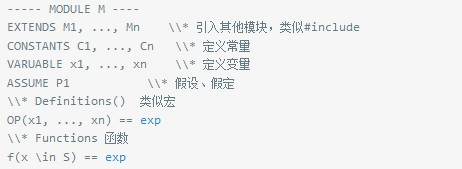
\includegraphics{figures/module.jpg}
\caption{TLA+编码模板}
\label{fig:graph}
\end{figure}

\subsection{TLA+ Modules}
TLA+ 提供了多种数据结构的实现,包括在本次实验中使用的sequecnce和record等。

record数据结构类似于C语言中的struct结构,即一个record包含若干个field,每个field可以在给定的集合中选取元素填充field。
sequence表示一个序列,如果引入Sequences模块,也可以将数组当作序列来进行处理,并且使用模块里的相应函数
在本次实验中,我们引入了TLA+ 中的Sequences模块,将List表示为一个Sequecnce,并且使用了如下的API:\\
\begin{tabular}{ccc}
\hline
operator& operation& example \\
\hline  
 Head& First element &Head(<<1, 2>>) = 1\\
 Tail& Sequence aside from head &Tail(<<1, 2>>) = <<2>>\\
 Append& Add element to end of sequence &Append(<<1>>, 2) = <<1, 2>>\\ 
 Len& Length of sequence &Len(<<1, 2>>) = 2\\
 $\backslash o$& Connect two sequences &<<1>>\ $\backslash o$\ <<2>> = <<1, 2>>\\
\hline % 
\end{tabular}
\par 以上的操作都不会使原有的操作序列发生变化。

\section{使用 TLA+ 描述 OT 函数}
解释同时描述并验证OT 函数。	 	
\subsection{LIST相关操作表示}
\subsubsection{第一、二类操作的表示}
采用record的数据结构来表示具体的操作。
第一类操作的record分为两种,set和ins有三个域:pos位置,ch操作字符,pr优先级。而del操作少了ch字符域,这样定义可以减少无效重复的操作数量,使验证代码的效率得到提高。
\begin{align*}
&OP\_1\_set \triangleq [type: {"set"}, pos: POS, ch: CH, pr:PR] \\
&OP\_1\_ins \triangleq [type: {"ins"}, pos: POS, ch: CH, pr:PR] \\
&OP\_1\_del \triangleq [type: {"del"}, pos: POS, pr:PR] \\
&OP\_1 \triangleq OP\_1\_set \cup OP\_1\_ins \cup OP\_1\_del\\
\end{align*}
第二类操作的record也分为两种,ins操作有三个域:pos插入位置,pr优先级,str要插入的字符串。del操作也有三个域:pos插入位置,pr优先级,len删除区间的长度
\begin{align*}
&OP\_2\_ins \triangleq [type: {"ins\_r"}, pos: POS, pr:PR, str:STR] \\
&OP\_2\_del \triangleq [type: {"del\_r"}, pos: POS, pr:PR, len:LEN] \\
&OP\_2 \triangleq  OP\_2\_ins \cup OP\_2\_del \\
\end{align*}

\subsubsection{第三类操作的表示}
第三类操作同样是使用record来表示,包含两个filed,即type类型和ints删除区间的集合。
\begin{align*}
OP\_3 \triangleq [type:{"del\_m"},ints:NoncoSeq] \\
\end{align*}

在表示第三类OT函数时,我们首先遇到的问题便是如何表示第三类List命令,由于第三类List命令为删除多个不相交的集合区间,因此我们需要使用TLA+遍历在List长度上所有可以表示出来的区间,一个命令的删除区间即为若干个不相交的符合条件的区间。
在TLA+中支持两个集合的笛卡尔积操作,因此所有符合条件的区间的集合Intervals可以如下定义:
\begin{align*}
Intervals \triangleq \{<a,b> \in POS \times POS: a+b \le Maxnum(POS)+1 \}
\end{align*}
a为区间的起始断点,b为区间长度,因为一个命令的删除区间为若干个不相交的符合条件的区间,定义区间后,便可以生成操作的删除区间。将一个删除操作的删除区间称为一个区间组合,那么有两种方式表示这种区间组合,一种是区间二元组的集合,另一种是二维数组,由于在接下来的OT函数中,需要较为方便地对操作进行转换,所以在本次实验中采用第二种表示方法,先生成第一种表示方法,即二元数组的集合。
\begin{align*}
& NoncoIntervals \triangleq \\ 
& \quad \{ints \in SUBSET \ Intervals : \forall i,j \in ints: i[2]+i[1] \le j[1] \lor j[2]+j[1] \le i[1] \lor i=j\} \backslash \{\{\}\}
\end{align*}
这样,$NoncoIntervals$中每个元素都是一个区间组合,下面我们需要将这个集合变成一个二维数组,由于在TLA+中没有执行某个指令固定次数的相应代码,所以在本次实验中需要多次使用递归来表示这种循环操作。一个符号在使用前必须先声明或者定义,所以使用递归要在函数或定义之前加上recursive关键字。
那么比如在这里我们需要将区间组合的集合转换为区间组合的数组,就需要使用两个递归的定义。
首先定义了将集合转化为序列的SetTOSeq():
\begin{align*}
RECURSIVE\ SetTOSeq(\_)\\
SetTOSeq(T) \triangleq &IF\ T =\ \{\}\ THEN <<>>\\
                       & ELSE\ LET\ t \triangleq CHOOSE\ x \in T : TRUE\\
                        & \quad IN\ <t>\ \backslash o\ SetTOSeq(T \backslash {t})\\
\end{align*}
接下来便可以定义Seqset(T),将二元组的集合的集合T转化为二维数组的集合:
\begin{align*}
&RECURSIVE Seqset(\_)\\
&Seqset(T) \triangleq  \\
& \quad IF\ T = {}\ THEN\ {}\\
& \quad ELSE\ LET\ t\triangleq\ CHOOSE\ x\ \in T : TRUE\\
& \quad IN\ Seqset(T \backslash {t}) \cup {SetTOSeq(t)} \\
&NoncoSeq\ \triangleq\ Seqset(NoncoIntervals)
\end{align*}
得到的集合$NoncoSeq$便为ints域的取值范围,这样遍历时得到的具体操作的ints域便为一个二维数组,该数组中横坐标表示第几个删除区间,纵坐标1的值表示该区间开始端带点,纵坐标为2的值表示区间长度。

\subsection{命令执行的表示}
命令的执行与LIST和具体操作相关,所以定义中使用的参数便是LIST和具体操作中的参数,使用Sequences模块中的API进行代码的编写。
以第二类的del操作为例,调用了 $\backslash o$和$SubSeq$定义:
\begin{align*}
del\_ran\_op(list,pos,len) \triangleq SubSeq(list, 1, pos-1) \quad \backslash o \quad SubSeq(list, pos+len, Len(list))
\end{align*}
唯一不同的是第三类操作的执行函数,同样是由于需要采用循环操作,所以还是要使用递归的定义完成命令的执行。
\begin{align*}
&RECURSIVE\ del\_mulran\_op(\_,\_,\_)\\
&del\_mulran\_op(list,ints,num) \triangleq \\
&  \quad  IF\ num = 0\ THEN\ list \\
&  \quad  ELSE\ del\_mulran\_op(SubSeq(list, 1, ints[num][1]-1)\ \backslash o\ SubSeq(list, ints[num][2]\\
&   \quad \quad  +ints[num[1],Len(list)),ints,num-1)    
\end{align*}
num是ints的区间个数,从后往前进行删除,这样不会影响下面要操作的区间,每次递归删除一个区间,并且值就是删除后的list,当num为0时就表示删除完成了,直接返回当前的参数中的list即可。

\subsection{OT函数的描述}
使用定义Xform表示OT函数,即Xform(lop, rop)为lop对于rop转换后的新操作。
以第一类函数为例:
\begin{align*}
&Xform(lop, rop) \triangleq \\
   & CASE \quad lop.type = "ins" \land rop.type = "ins" -> Xform\_ins\_ins(lop, rop)\\
   & []  \quad lop.type = "ins" \land rop.type = "del" -> Xform\_ins\_del(lop, rop)  \\
   & [] \quad  lop.type = "ins" \land rop.type = "set" -> Xform\_ins\_set(lop, rop)  
\end{align*}
\subsubsection{第一类函数的表示}
第一类函数的表示较为简单,不需要使用递归结构。
以$ins$操作对于$ins$操作的转换来举例说明,使用定义$Xform\_ins\_ins$表示OT函数,即$Xform\_ins\_ins(lins, rins)$为$ins$操作对于$ins$操作转换后的新操作。
\begin{align*}
&Xform\_ins\_ins(lins, rins) \triangleq \\
    &\quad IF \quad lins.pos < rins.pos\\
    &\quad THEN \quad lins\\
    & \quad \quad ELSE \quad IF \quad lins.pos > rins.pos\\
        & \quad \quad \quad THEN \quad [lins \quad EXCEPT !.pos = @ + 1]\\
        & \quad \quad \quad ELSE \quad IF \quad lins.pr < rins.pr\\
                &\quad \quad \quad \quad THEN \quad [lins \quad EXCEPT !.pos = @+1]\\
                &\quad \quad \quad \quad ELSE \quad  lins
\end{align*}
其中EXCEPT !的意思为除了特定的域发生变化,其他域保持不变。
这样参照着之前第一类函数的数学公式,便可以类似地将其他第一类函数用同样的方式表示出来。
\subsubsection{第二类函数的表示}
第二类函数的表示也比较简单,同样不需要使用递归结构。
以$ins$操作对于$del$操作的转换来举例说明,使用定义$Xform\_ins\_del\_r$表示OT函数,即$Xform\_ins\_del\_r(ins, del)$为$ins$操作对于$del$操作转换后的新操作。
\begin{align*}
&Xform\_ins\_del\_r(ins,del) \triangleq \\
   & \quad CASE ins.pos \le del.pos -> ins \\
   & \quad [] ins.pos > del.pos \land ins.pos < del.pos + del.len -> NOP \\
   & \quad [] ins.pos \ge del.pos + del.len -> [ins \quad EXCEPT !.pos = @ - del.len] 
\end{align*}
EXCEPT !的意思为除了特定的域发生变化,其他域保持不变。
这样参照着之前第二类函数的数学公式,便可以类似地将其他第二类函数用同样的方式表示出来。
\subsubsection{第三类函数的表示}
第三类函数为第三类的Del命令与第二类命令中的Ins操作之间的OT函数,以及第三类Del命令自身的OT函数,共2+1=3个。
这类函数的设计代码量占到了整个设计的一半,大量使用了递归定义,这里拿最为复杂的Del命令自身的OT函数来举例。
\begin{align*}
&RECURSIVE\ Xform\_del\_del\_m(\_,\_,\_)\\
&Xform\_del\_del\_m (ldel,rdel,i) \triangleq \\
& \quad IF\ i > Len(ldel.ints)\ THEN\ ldel\\
& \quad \quad  ELSE\ Xform\_del\_del\_m ([ldel\ EXCEPT !.ints[i]= transdel4(@,rdel.ints)],rdel,i+1)
\end{align*}
使用定义$Xform\_del\_del\_m$表示OT函数,这里设置i为递归变量,i为ldel中当前正在进行转换的区间,转换函数为transdel4,按照公式(3-10)进行编写,即进行一个删除区间相对于rdel的转换,这样当i的值大于ldel中删除区间的数量时,所有删除区间都完成了转换,将转换后的新区间合并起来,便是ldel转换后的新操作。
\begin{align*}
&transdel4(int,ints) \triangleq \\ 
  & \quad <<newpos(int[1],ints,1),newlen(int[1],int[2],ints,1,0)   >>
\end{align*}
$newpos$和$newlen$便是这个删除区间对于rdel的转换后的新区间端点和区间长度。
$newpos$和$newlen$两个定义同样使用递归结构来表示。
$newpos$:
\begin{align*}
& RECURSIVE newpos(\_,\_,\_)\\
& snewpos(pos,ints,i) \triangleq\\
&\quad IF  pos < ints[1][1] THEN pos\\
&\quad ELSE IF i=Len(ints) \land pos \ge ints[i][1] + ints[i][2] THEN pos - Dlen(ints,i,0)\\
&\quad ELSE IF pos \ge ints[i][1] \land pos < ints[i][1] + ints[i][2] THEN ints[i][1] - Dlen(ints,i-1,0)\\
&\quad ELSE IF ints[i][1] + ints[i][2] \le pos \land pos < ints[i+1][1] THEN pos - Dlen(ints,i,0)\\
&\quad ELSE newpos(pos,ints,i+1)
\end{align*}
递归变量为i,代表当前在对rdel中第几个区间进行newpos的计算,每递归一次,i的值加一,如果满足条件要求则返回相应newpos的值。其中Dlen的作用为统计rdel中前i个删除区间的长度之和(代码详见附录)。
$newlen$:
\begin{align*}  
&RECURSIVE newlen(\_,\_,\_,\_,\_)     \\
&newlen(pos,len,ints,i,sum) \triangleq\\
    & \quad IF\ i > Len(ints) \ THEN \quad len - sum\\
    & \quad ELSE \ IF \ pos + len < ints[i][1] \ THEN \ newlen(pos,len,ints,i+1,sum)\\
    & \quad ELSE \ IF \ pos < ints[i][1] \land ints[i][1] < pos + len \land pos + len \le ints[i][1] + ints[i][2]\\
    & \quad \quad THEN \ newlen(pos,len,ints,i+1,sum + pos + len -ints[i][1])\\
    & \quad ELSE \ IF \ pos < ints[i][1] \land pos + len > ints[i][1] + ints[i][2]\\
    & \quad \quad THEN \ newlen(pos,len,ints,i+1,sum + ints[i][2])\\
    & \quad ELSE \ IF \ ints[i][1] \le pos \land pos < ints[i][1] + ints[i][2] \land pos + len \le ints[i][1] + ints[i][2]\\
    & \quad THEN \ 0\\
    & \quad ELSE \ IF\ ints[i][1] \le pos \land pos < ints[i][1] + ints[i][2] \land pos + len > ints[i][1] + ints[i][2] \\
    & \quad \quad THEN \ newlen(pos,len,ints,i+1,sum + ints[i][1] + ints[i][2] - pos)    \\
    & \quad ELSE \ newlen(pos,len,ints,i+1,sum)
\end{align*}
递归变量为i和sum,i表示当前在对rdel中第几个区间进行newlen的计算,sum表示在当前计算完成的所有区间中len转换为newlen需要减去的长度。
这样便根据公式(3-10)完成了Del命令自身的OT函数,第三类的Del命令与第二类命令中的Ins操作之间的OT函数可以用类似地方式表示出来,同时,剩余的OT函数也可以用递归或非递归的形式根据公式进行表示,在此不再赘述。
\section{正确性验证}
上节中已经完成了OT函数的TLA+描述,剩下的就是决定验证的目标和方式。
验证的目标: CP1 如何用 TLA+ 表示。

我们验证CP1性质的正确性。即同一个List经过OT(OP2,OP1),OP1或者OT(OP1,OP2),OP1这两种操作序列后,最终的结果是一致的。
结合以上给出的定义,用TLA+来描述所设计OT函数的CP1正确性:
\begin{align*}
  apply(apply(list,op1),Xform(op2, op1)) = apply(apply(list,op2),Xform(op1, op2))
\end{align*}
\par 只要对于任意的两个操作,这个等式都成立的话,那么CP1正确性即可得到验证。

因为在本次实验中不涉及系统状态的变化,只需证明等式对于所有操作都成立即可,因此没有behavior spec,即没有初始状态 Init 和状态关系 Next。不过,在TLC中提供了Evaluate Constant Expression的功能,即可以计算常量表达式的值。以第一类函数的CP1验证为例,我们给出如下正确性定义:
\begin{align*}
 & correctness_1 (list) ==\\
 & \quad \forall op1,op2 \in OP_1:\\
 & \quad \quad \lor op1.pr = op2.pr\\
 & \quad \quad \lor apply(apply(list,op1),Xform(op2, op1)) = apply(apply(list,op2),Xform(op1, op2))  
\end{align*}
这样的话,$op1$,$op2$就实现了对$OP_1$中所有操作的遍历,并且对于满足要求的任意$op1$和$op2$,只要优先级满足要求(两个操作的优先级不相等),则其一定满足CP1等式。
在Evaluate Constant Expression内填写这个表达式,我们便可以check model并根据value的值来检验函数的正确性了。

\subsection{TLA+ Model Checker 设置及实验环境}
在本次实验中,我们定义Model Checker中常量的参数值如下:\\
STR <- {"like","enjoy","fond","love","fantasy"} \\
CH <- {"a","b","c","d","e"}\\
PR <- {1,2}\\
STR为第二类插入操作中str域的可选择范围,CH为第二类插入、设置操作中ch域的可选择范围,PR为操作的优先级,在此处我们设定两个操作的优先级不相同,否则为违规操作变换。
通过调整LIST常量的长度,实验在不同长度的LIST下完成各类函数的验证所需要的时间。

实验环境:\\
Number of worker threads: 12\\
Fraction of physical memory allocated to TLC: 16173 mb

\subsection{实验结果}
\begin{figure}[H]
\centering
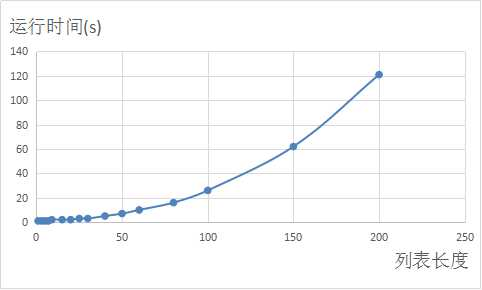
\includegraphics{figures/runtime1.bmp}
\caption{验证第一类函数正确性的运行时间与列表长度(横坐标)的关系}
\end{figure}
\par 结果分析:若列表长度为n,则第一类操作的个数:$5*2*n(ins)+5*2*n(set)+2*n(del) = 22n$
任意选取其中两个操作验证CP1正确性,所以验证算法的时间复杂度为$O(n^2)$
从实验结果看,与复杂度的分析相一致。

\begin{figure}[H]
\centering
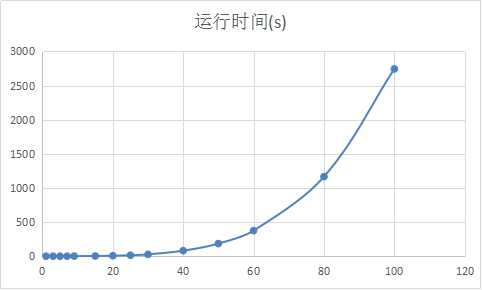
\includegraphics{figures/runtime2.bmp}
\caption{验证第二类函数正确性的运行时间与列表长度(横坐标)的关系}
\end{figure}
\par 结果分析:若列表长度为n,则第二类操作的个数:$5*2*n(ins))+n*2*n(del) = 2n^2+10n$
任意选取其中两个操作验证CP1正确性,所以验证算法的时间副复杂度为$O(n^4)$
从实验结果看,与复杂度的分析相一致。

\begin{figure}[H]
\centering
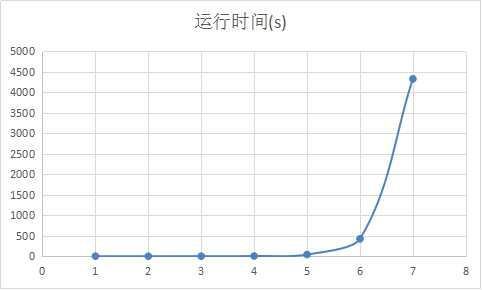
\includegraphics{figures/runtime3.bmp}
\caption{验证第三类函数正确性的运行时间与列表长度(横坐标)的关系}
\end{figure}
\par 结果分析:目前第三类函数的验证结果只能到LIST长度为7。
因为第三类操作的个数为指数级别$O(3^n)$,并且在生成操作和操作的转换过程中多次使用了递归,更大大增加了验证算法的复杂程度。

\begin{figure}[H]
\centering
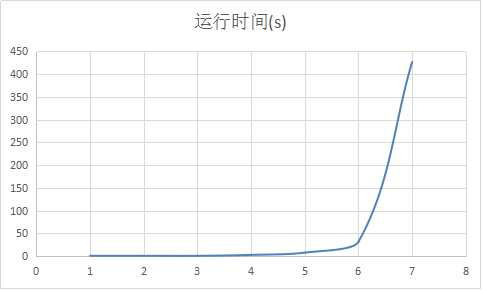
\includegraphics{figures/runtime4.bmp}
\caption{验证其余函数正确性的运行时间与列表长度(横坐标)的关系}
\end{figure}
\par 结果分析:目前其余函数的验证结果只能到LIST长度为7。
与第三类函数的验证相同,在其余函数的验证算法中也需要生成$O(3^n)$级别的第三类操作和使用递归代码实现操作的转换,因此复杂度与第三类函数相仿。

\begin{figure}[H]
\centering
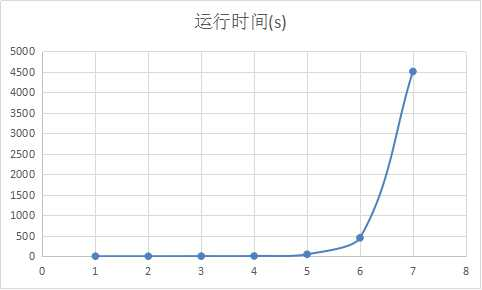
\includegraphics{figures/runtimeall.bmp}
\caption{验证所有OT函数正确性与列表长度(横坐标)的关系}
\end{figure}
\par 结果分析:时间复杂度与第三类函数的复杂度相同,目前可以验证所设计的OT函数在LIST长度为7之内时的正确性。
	%未来工作
	\chapter{结论与未来工作}
\par Redis List命令的OT函数设计经过验证是成功的。
\section{工作总结}

\section{研究展望}

	%参考文献
	\bibliography{thesis}
	%致谢
	\begin{acknowledgement}
  本文的工作是在魏恒峰老师的悉心指导下完成的。
  魏老师严谨的治学态度和认真的工作态度给了我极大的影响。
  在相关知识的学习、实验过程以及论文的写作过程中,魏老师也给了我莫大的帮助。
  在此衷心感谢魏老师这半年的关心和指导。

感谢黄宇老师和马晓星老师,他们在我的学习和实验过程中也给出了很多宝贵的指导和建议。

感谢我的同学们,很幸运能与易星辰、王芷芙、唐瑞泽等同学在 TLA+ 讨论班中共同学习和进步。
感谢黄羿学长,张宇奇学长在我实验过程中给与的帮助和指导。
感谢缪娅,谢谢你的理解和陪伴。

感谢我的父母,谢谢你们一直关心着我,一直给我无私的爱。
你们的支持是我顺利完成学业的最大动力。
\end{acknowledgement}
	%附录
	\chapter{附录} 
\section{OT函数的设计}
\subsection{第一类 OT 函数的设计}
第一类函数为第一类命令之间的OT函数,即Ins,Del,Set三种操作之间的OT函数,共有3*3=9个。
\begin{equation}
\begin{aligned}
Set \begin{cases}
OT(set (i,x), set (j,y)) =\begin{cases}
    no-op \quad &pr1 > pr2 \quad i=j\\
	{set (i,x)} \quad &else \end{cases} \\ 
OT(Set(i,x),Ins(j,y))=\begin{cases}
{Set(i,x)}  \quad &i<j\\
{Set(i+1,x)} \quad  &i\ge j \end{cases} \\
OT(Set(i,x),Del(j))=\begin{cases}
{Set(i,x)} \quad &i<j\\
{no-op} \quad & i=j\\
{Set(i-1,x)} \quad &i>j \end{cases} \\
\end{cases}
\end{aligned}
\end{equation}
\begin{equation}
\begin{aligned}
Ins \begin{cases}
OT(Ins(i,x), set (j,y)) =
{Ins(i,x)}\\
OT(ins (i,x), ins (j,y)) =\begin{cases}
	{ins(i+1, x)}   \quad & i > j\\
	{ins(i, x)}    \quad & i < j\\
	{ins(i+1, x)}   \quad  & i = j \quad pr1 < pr2\\
	{ins(i, x)}   \quad  & i = j \quad pr1 > pr2 \end{cases} \\
OT(Ins(i,x),Del(j))=\begin{cases}
{Ins(i,x)}  \quad i \le j\\
{Ins(i-1,x)} \quad i>j \end{cases}\\
\end{cases}
\end{aligned}
\end{equation}


\begin{equation}
\begin{aligned}
Del \begin{cases}
OT(Del (i), Set (j,x)) =
	{Del(i)}\\
OT(Del (i), Ins (j,x)) =\begin{cases}
	{Del (i+1)}  \quad &i \ge j\\
	{Del (i)}   \quad &i < j\\ \end{cases}\\
OT(del (i), del (j)) =\begin{cases}
	{Del (i-1)} \quad &i > j\\
	{Del (i)} \quad &i < j\\
	{no-op}   \quad &i = j \end{cases}\\
\end{cases}
\end{aligned}
\end{equation}

\subsection{第二类 OT 函数设计}
第二类函数为第二类命令之间的OT函数,即Ins,Del两种命令之间的OT函数,共2*2=4个。
\begin{equation}
OT(Ins(p1,s1),Ins(p1,s2))= \begin{cases}
Ins(p1,s1) \quad & p1<p2 \\
Ins(p1+ |s2|,s1) \quad & p1>p2 \\
Ins(p1+ |s2|,s1) \quad & p1=p2 \quad pr1<pr2 \\
Ins(p1,s1) \quad & p1=p2 \quad pr1>pr2
 \end{cases}\\
\end{equation}

\begin{equation}
OT(Ins(p1,s1),Del(p2,l1))= \begin{cases}
Ins(p1,s1) \quad & p1 \le p2 \\
no-op \quad & p2<p1<p2+l1\\
Ins(p1-l1,s1) \quad & p1 \ge p2+l1 \end{cases}\\
\end{equation}

\begin{equation}
OT(Del(p1,l1),Ins(p2,s1))= \begin{cases}
Del(p1,l1) \quad & p1 + l1 \le p2 \\
Del(p1,l1+|s1|) \quad & p1<p2<p1+l1 \\
Ins(p1+ |s1|,l1) \quad & p1 \ge p2 \end{cases}\\
\end{equation}

\begin{equation}
OT(Del(p1,l1),Del(p2,l2))= \begin{cases}
Del(p1,l1) \quad & p1<p2 \quad p1+l1 \le p2 \\
Del(p1,p2-p1) \quad & p1<p2 \quad p2<p1+l1 \le p2+l2\\
Del(p1,l1-l2) \quad & p1<p2 \quad p2+l2<p1+l1\\
no-op \quad & p2 \le p1 < p2+l2 \quad p1+l1 \le p2+l2\\
Del(p2,p1+l1-p2-l2) \quad & p2 \le p1 <p2+l2 \quad  p1+l1>p2+l2\\
Del(p1-l2,l1) \quad & p1 \ge p2+l2  \end{cases}\\
\end{equation}

\end{document}